\documentclass[UKenglish]{beamer}


\usepackage[utf8]{inputenx} % For æ, ø, å
\usepackage{csquotes}       % Quotation marks
\usepackage{microtype}      % Improved typography
\usepackage{amssymb}        % Mathematical symbols
\usepackage{mathtools}      % Mathematical symbols
\usepackage[absolute, overlay]{textpos} % Arbitrary placement
\setlength{\TPHorizModule}{\paperwidth} % Textpos units
\setlength{\TPVertModule}{\paperheight} % Textpos units
\usepackage{tikz}
\usetikzlibrary{overlay-beamer-styles}  % Overlay effects for TikZ

\usepackage{hyperref}
\usepackage{svg}

\usepackage{color, soul, xcolor} % Colored text and highlighting, respectively
\usepackage{tikz-cd} % For commutative diagrams
\usepackage{tikz-3dplot}
\usetikzlibrary{angles}
\RequirePackage{pgfplots}
\usepackage{mathtools}
\usepackage{answers}
\usepackage{setspace}
\usepackage{graphicx}
\usepackage{enumerate}
\usepackage{multicol}
\usepackage{mathrsfs}
\usepackage{amsmath,amsthm,amssymb}
\usepackage{marvosym,wasysym} %fucking smileys
\usepackage{float}
\usepackage{morefloats}
\usepackage{pgf,tikz}
\pgfplotsset{compat=1.15}
\usepackage{mathrsfs}
\usetikzlibrary{arrows}
\usepackage{subcaption}
\usepackage[most]{tcolorbox}
\tcbuselibrary{theorems}
\usepackage{fancyvrb}
\usepackage{longtable,booktabs}
\usepackage{stackrel}


\usetheme{UiB}


\author{Leah Gibson \& Colin Roberts}
\setbeamercolor{title}{fg=white} 
\title{Spherical Geometry}
\setbeamercolor{subtitle}{fg=white} 
\subtitle{Windsor Charter Academy}


\begin{document}

\begin{frame}{Question}
    What do we know about geometry?
\end{frame}


\begin{frame}{Question}
    Which is the shortest path between the two points?
    \pause
    \begin{figure}[H]
  \centering
  \includesvg[width=.7\textwidth]{Figures/which_is_shortest.svg}
    \end{figure}
    Draw your answer on a white board.
\end{frame}

\begin{frame}{Answer}
    Straight line!
    \vspace*{2.5cm}
        \begin{figure}[H]
  \centering
  \includesvg[width=.7\textwidth]{Figures/which_is_shortest_ans.svg}
    \end{figure}
\end{frame}

\begin{frame}{Question}
    What if instead of drawing on rectangular board, we draw on a ball?
    \vfill
    \pause
    Think of it this way:\\
    
    \pause
    What is the shortest path between two cities on Earth? 
\end{frame} 

\begin{frame}{Answer}
    Great circles!
    \vfill
    \begin{figure}[H]
        \centering
        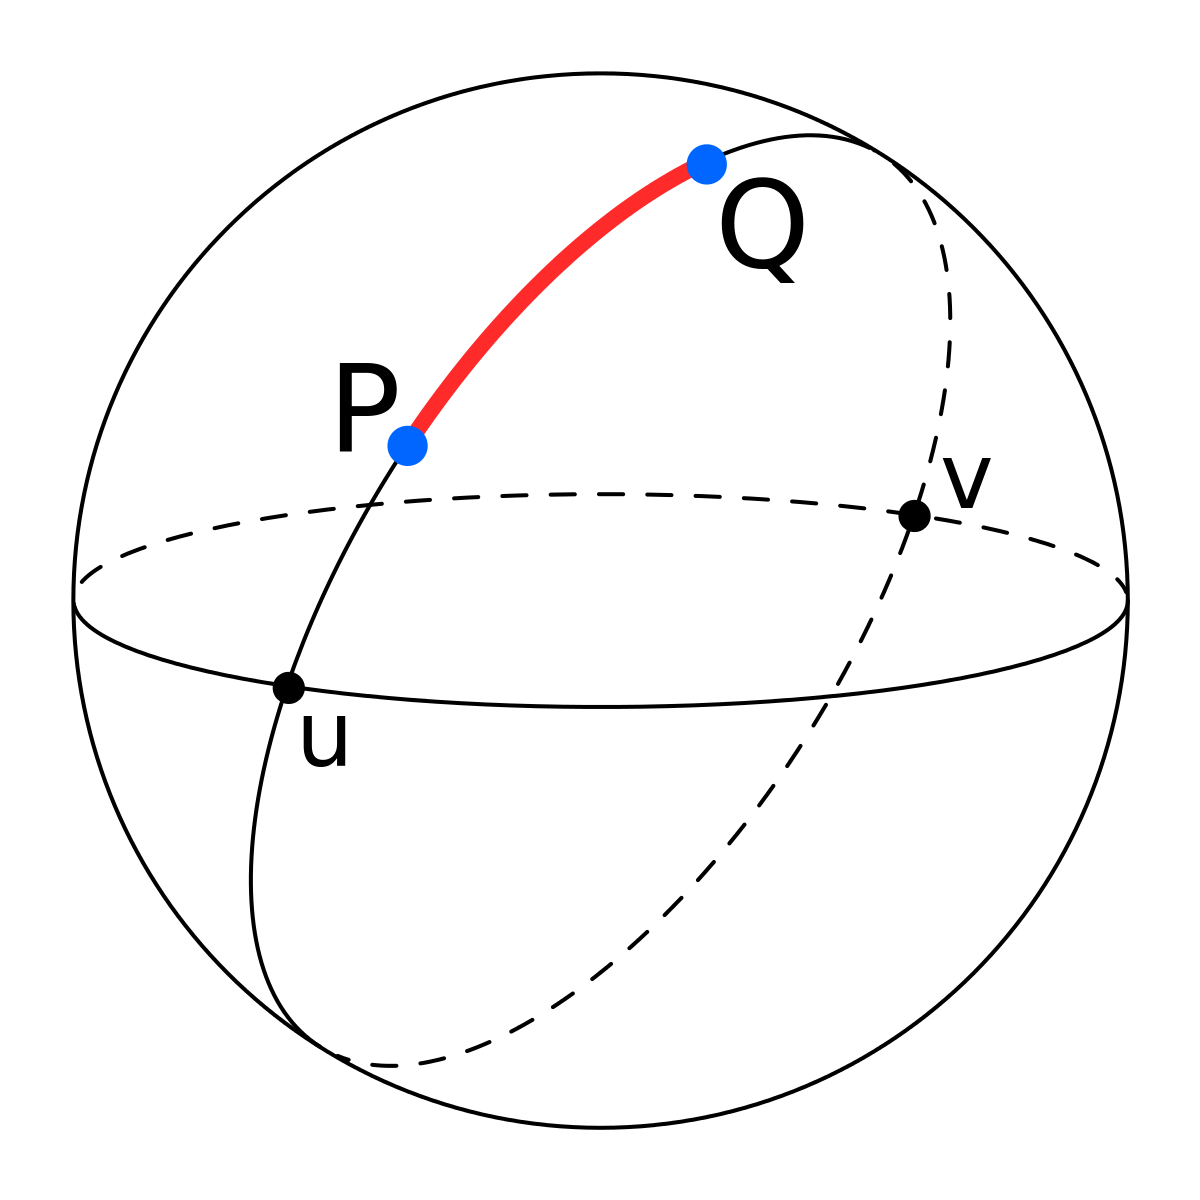
\includegraphics[width=.6\textwidth]{Figures/great_circle.png}
    \end{figure}
\end{frame}

\begin{frame}{Activity}
    Draw the shortest paths on spheres!\\
    
    \begin{enumerate}[1.]
        \item Pick two points on your sphere and draw what you think is the shortest path between the two points.
        \item Check if you're right by putting your rubber band around the sphere on the line that you drew.
        %other idea/troubleshooting: show them what the rubber band should look like or use transparent half spheres that Mark has
    \end{enumerate}
    
    %Allow 5 min for activity
    
    
\end{frame}


% \begin{frame}{Mercator Projection}
%     \begin{figure}[H]
%         \centering
%         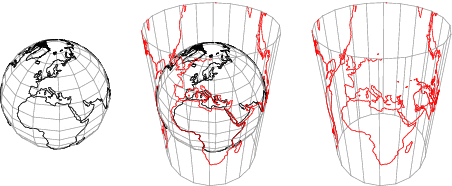
\includegraphics[width=.5\textwidth]{Figures/CylindricalProjection3D_700.png}
%     \end{figure}
%     \begin{figure}[H]
%         \centering
%         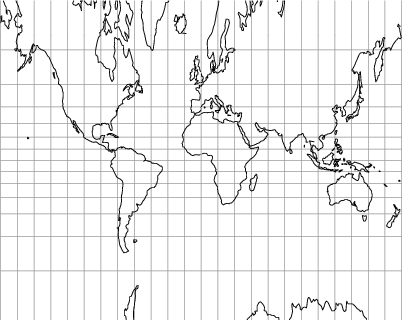
\includegraphics[width=.5\textwidth]{Figures/CylindricalProjection_1000.png}
%     \end{figure}
% \end{frame}




\begin{frame}{Question}
    Can you draw a triangle with all 90$^\circ$ angles on paper?\\
    \pause
    Give this a try on your white board.
\end{frame}

\begin{frame}{Answer}
    No! 
    \pause
    There must be 3 angles that have a total of 180$^\circ$!
\end{frame}

\begin{frame}{Triangles in the Plane}
    We have these types of triangles in the plane.
    \begin{figure}
        \centering
        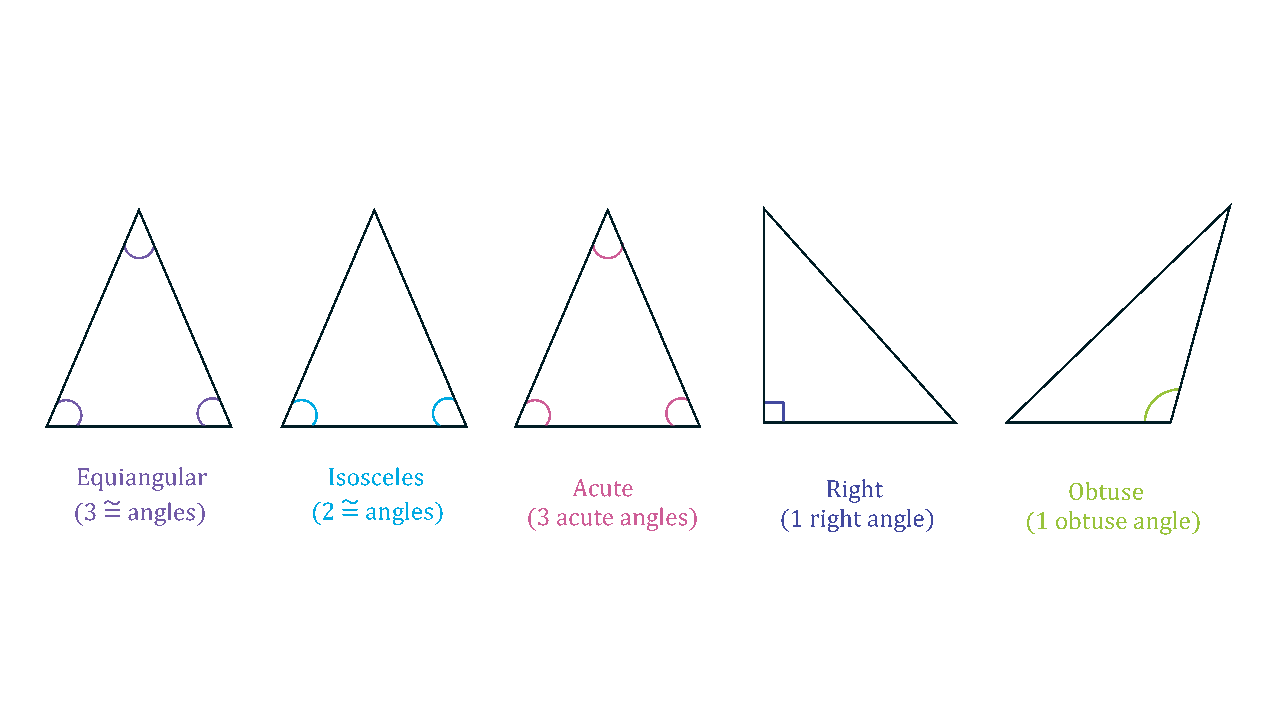
\includegraphics[width=.7\textwidth]{Figures/triangle-classification-angles.png}
    \end{figure}
\end{frame}

\begin{frame}{Question}
    What if we tried this on a sphere?
\end{frame}


\begin{frame}{Activity}
    Draw triangles using great circles on the sphere, and add up their total angles!\\
    \vspace*{2cm}
    Can you draw a triangle with three 90$^\circ$ angles on the sphere?
    %Ideas: use rubber bands to construct great circles
    %If they don't do it, we show triangle with 3 right angles
\end{frame}


%% TIME PERMITTED?

\begin{frame}{Shortest path}
How do planes fly over Earth?
\pause
        \begin{figure}[H]
        \centering
        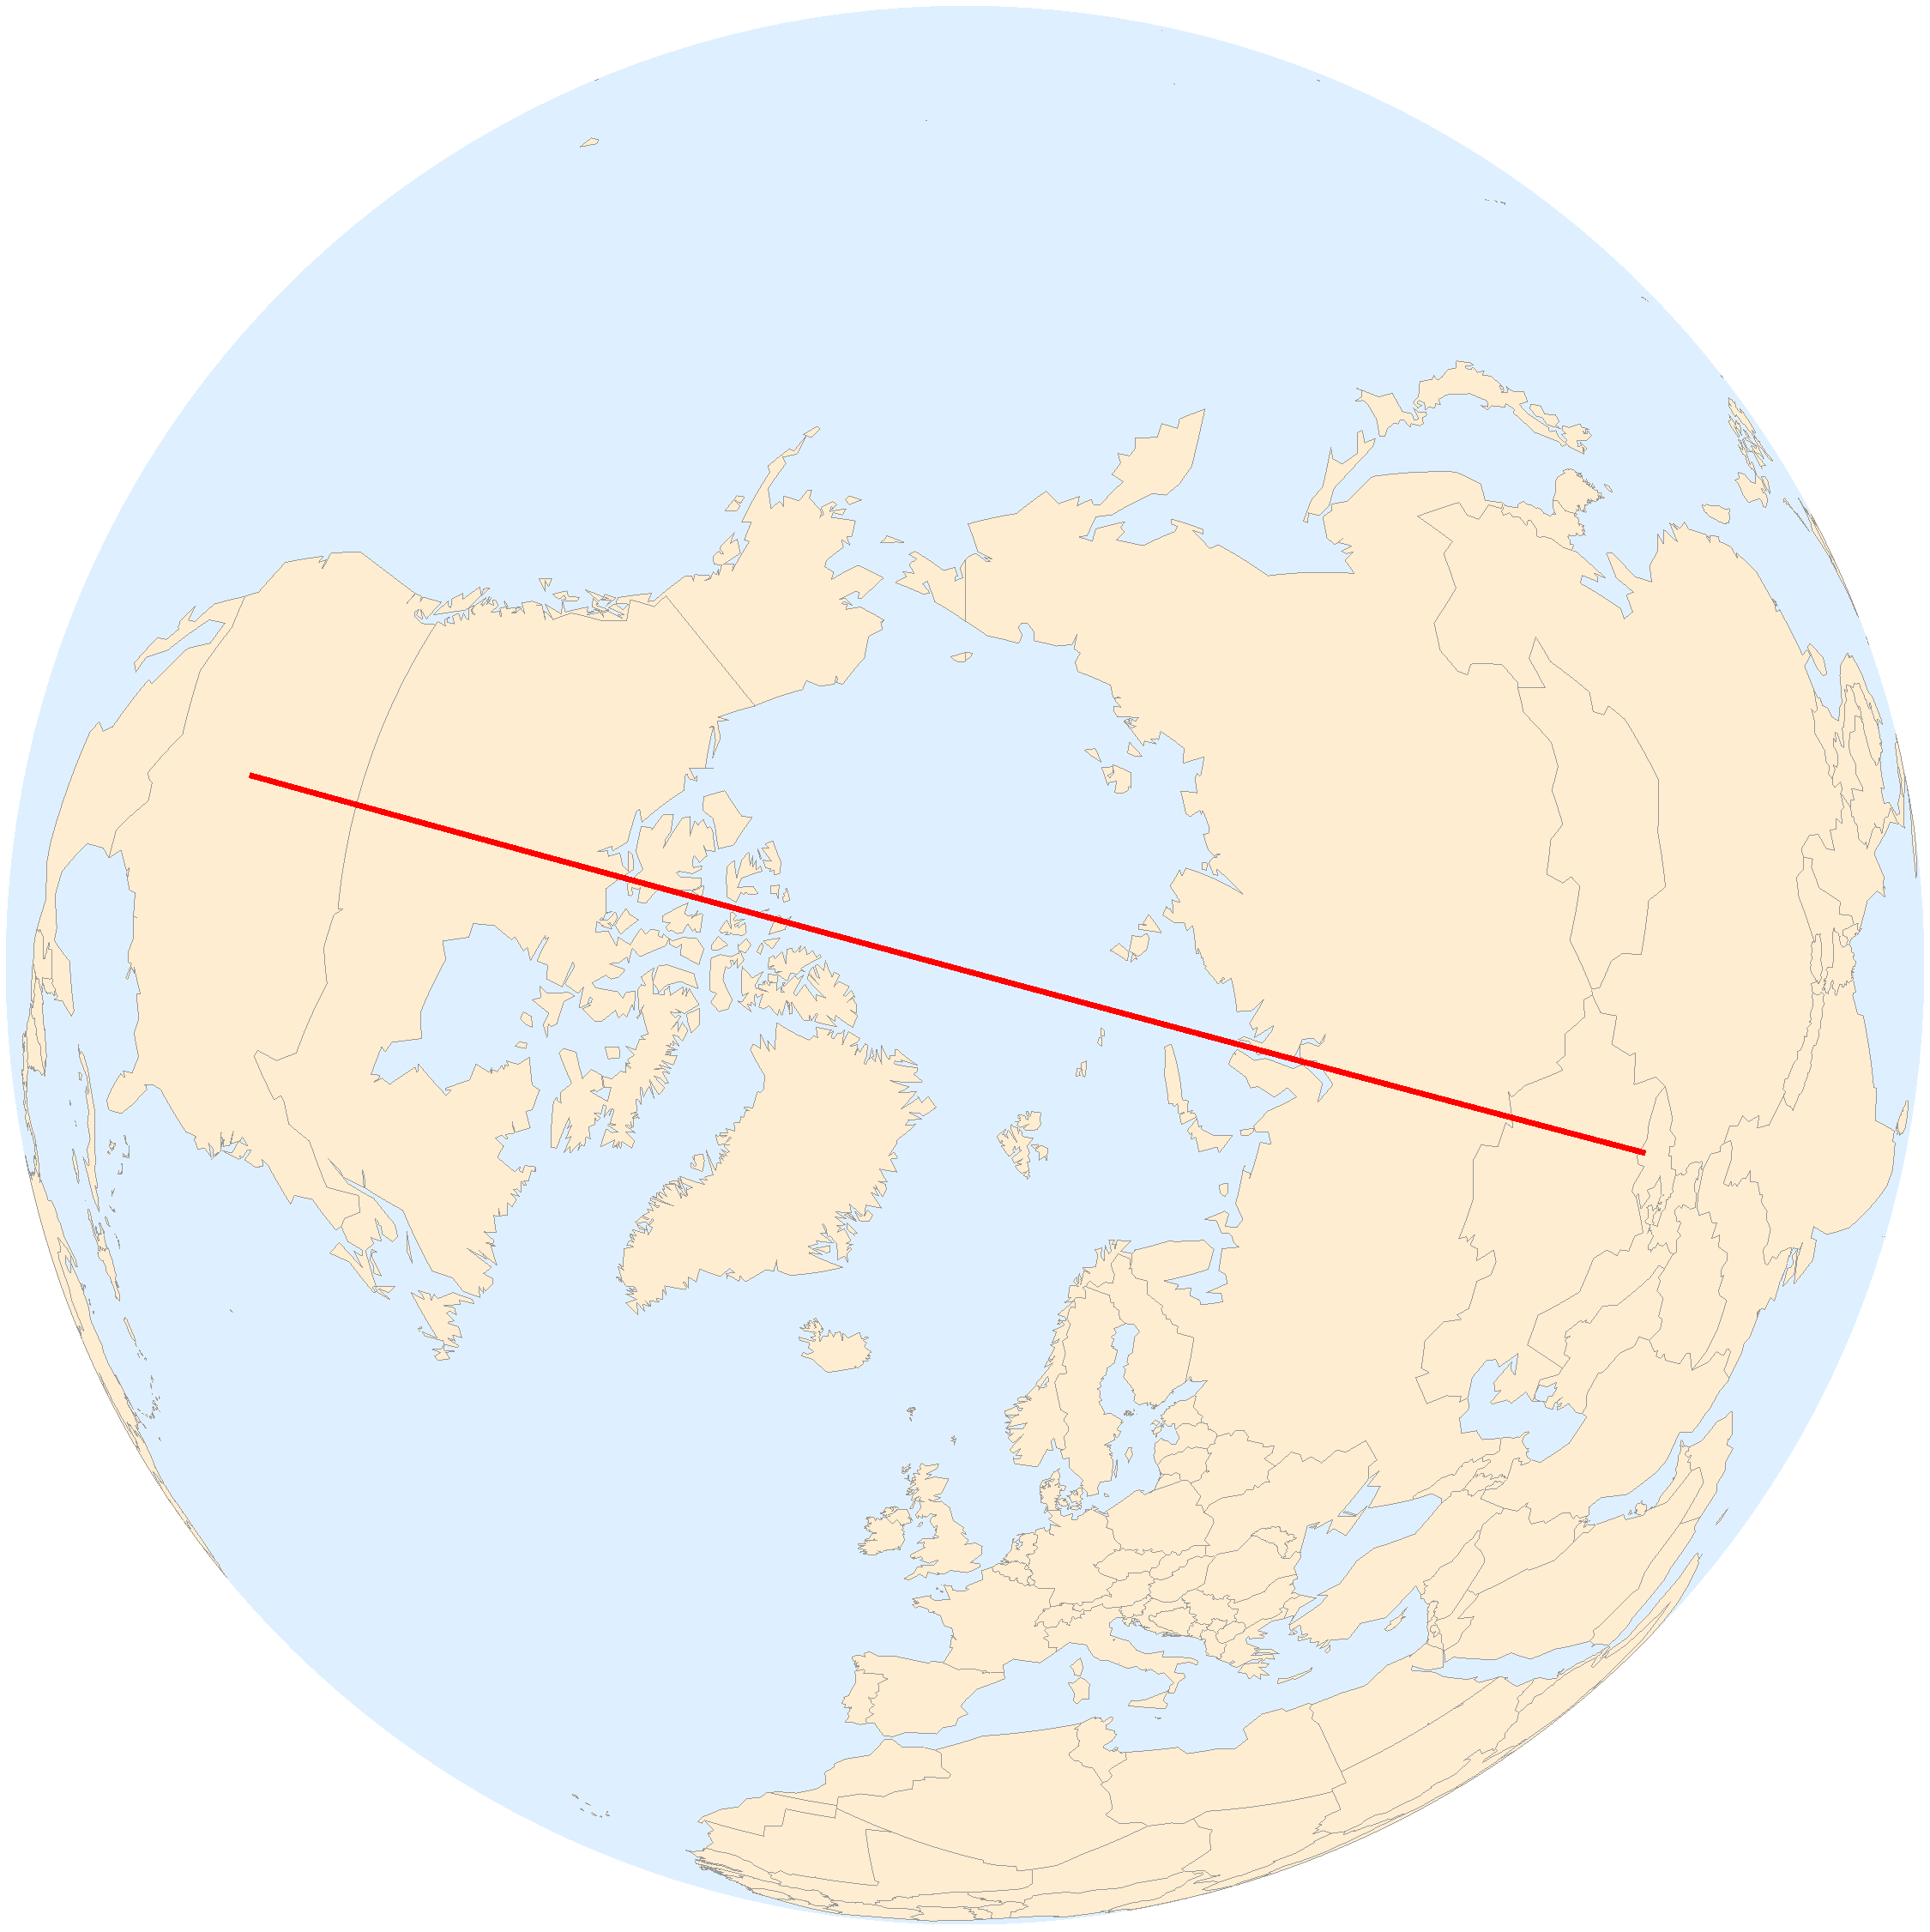
\includegraphics[width=.6\textwidth]{Figures/earth_two_cities.pdf}
    \end{figure}
\end{frame}

\begin{frame}{Activity}
    Name two cities and we can the plane flight between them and see what this looks like on the map!
\end{frame}

\begin{frame}{On a Map}
Here is what a bunch of flights look like on a map.
    \begin{figure}
        \centering
        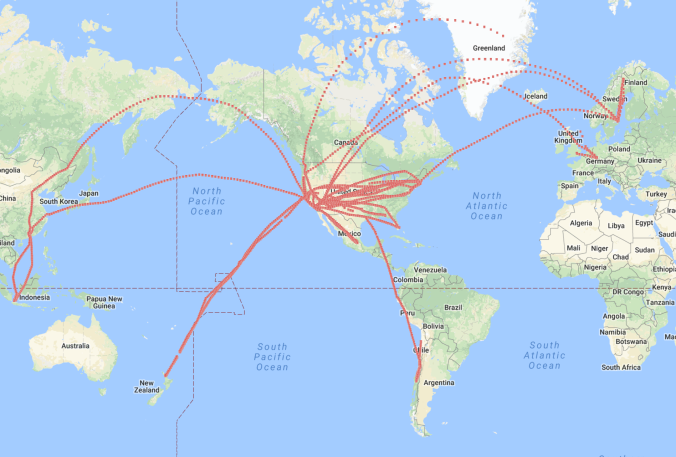
\includegraphics[width=.8\textwidth]{UiB-images/flightpaths.png}
    \end{figure}
\end{frame}

\begin{frame}{On a Map}
Why do these lines not look straight on a map?
    \begin{figure}[H]
        \centering
        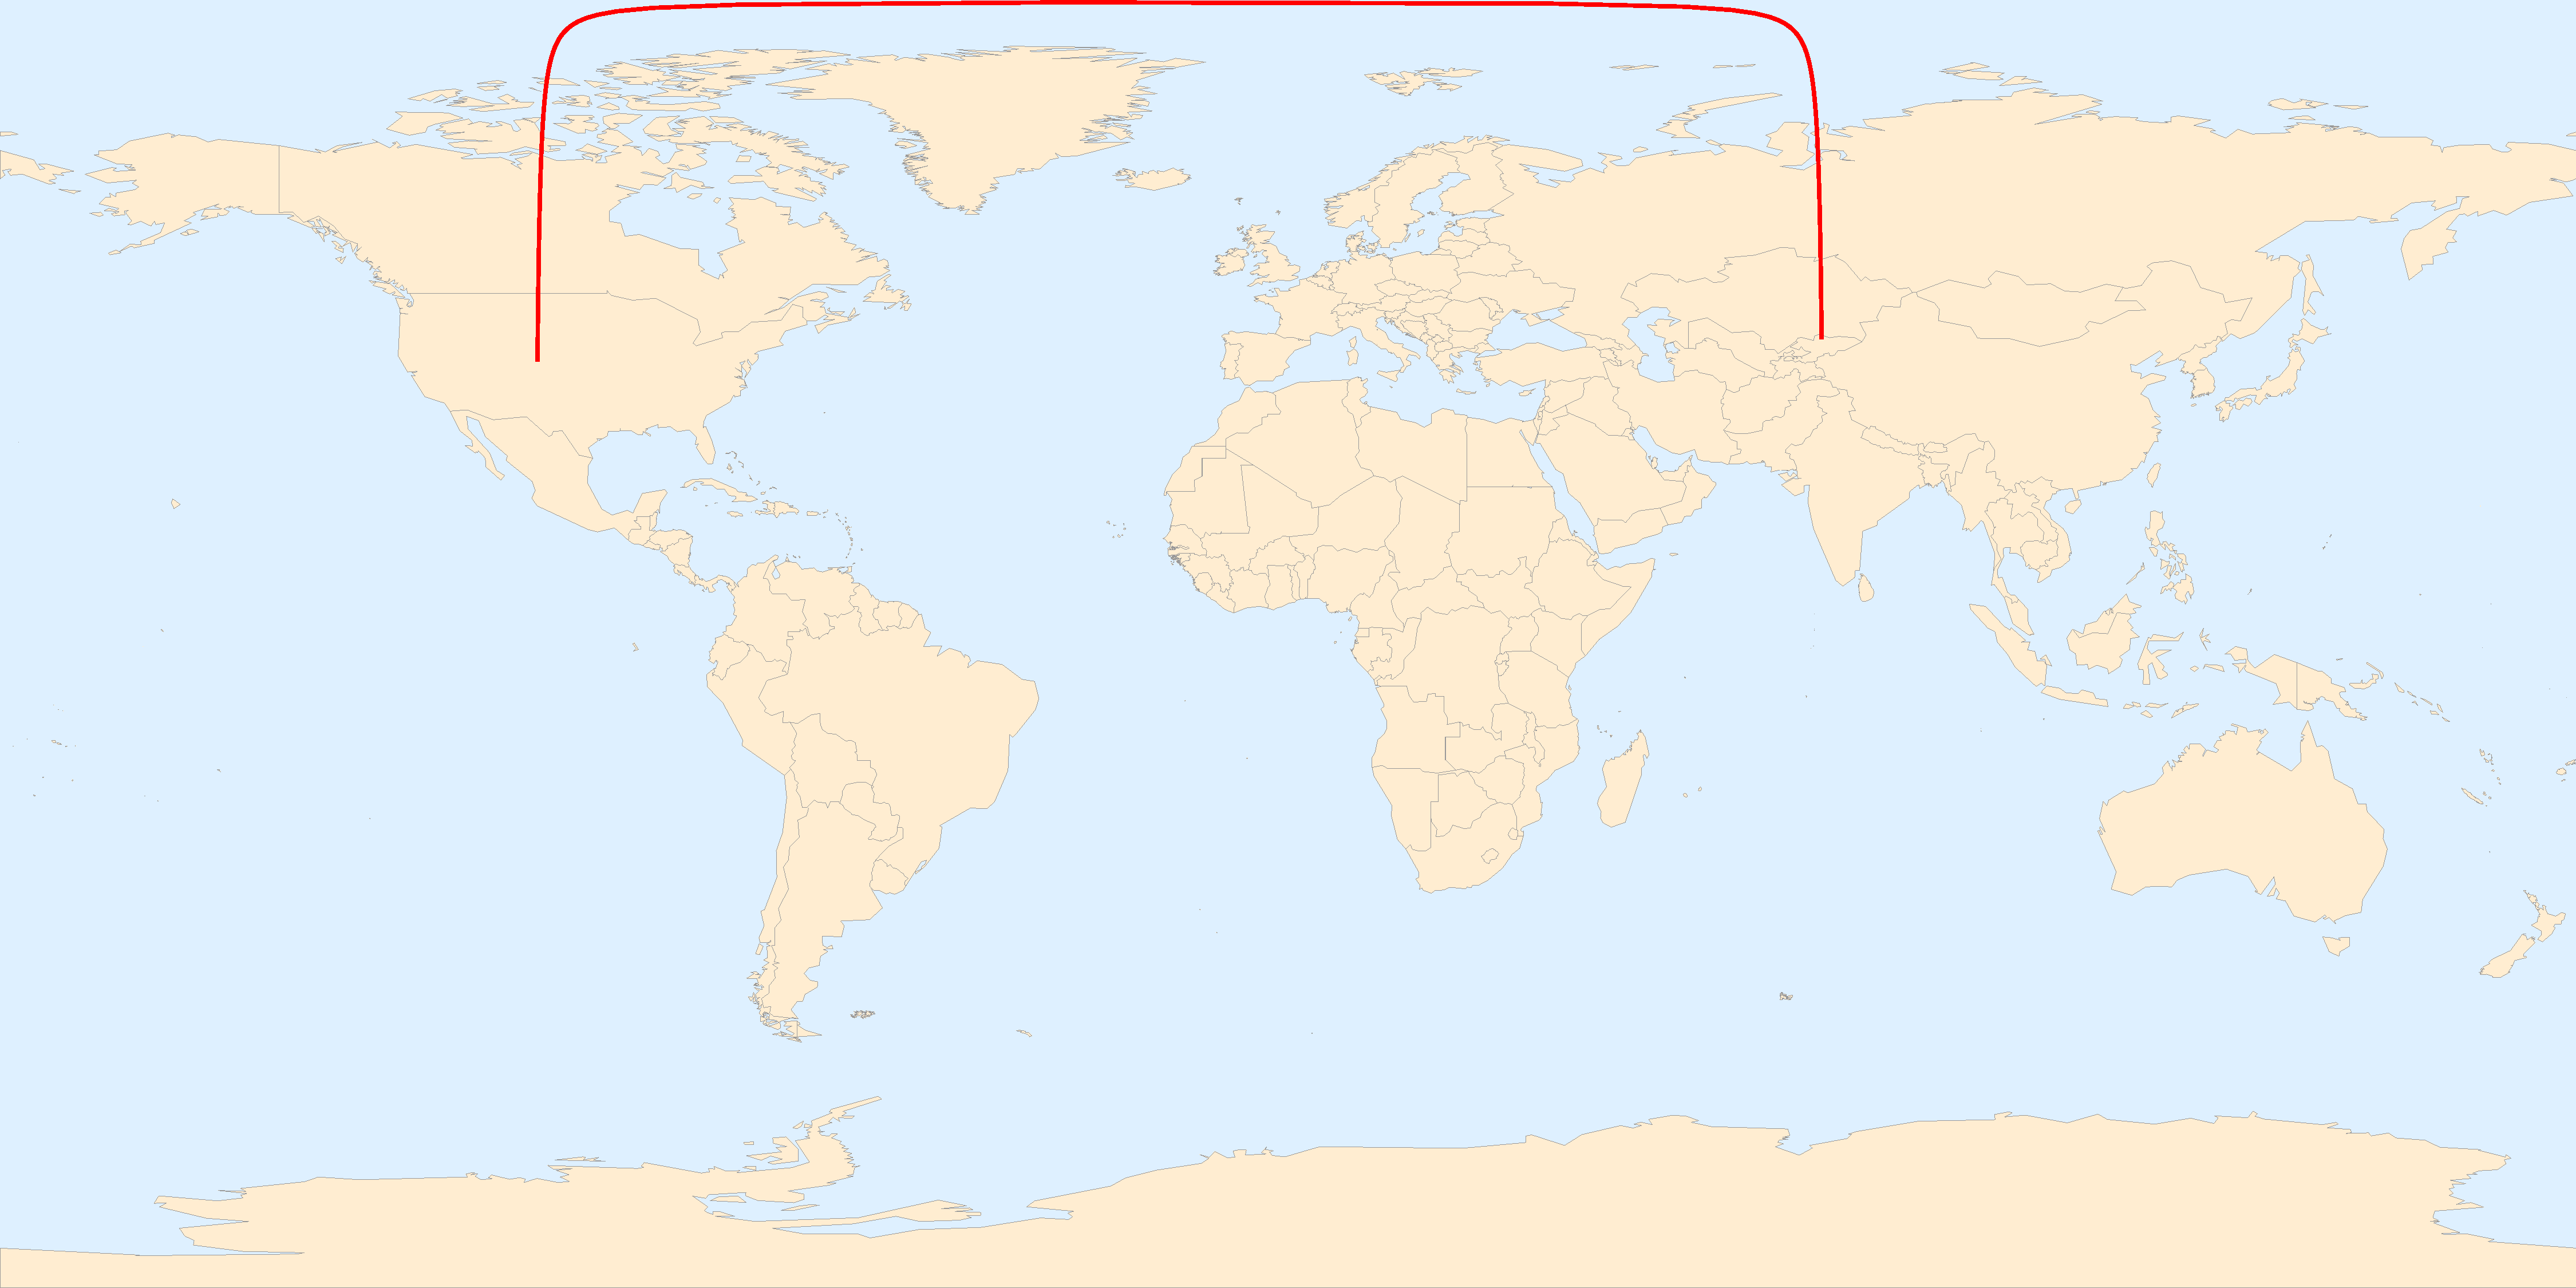
\includegraphics[width=.9\textwidth]{Figures/mercator_two_cities.pdf}
    \end{figure}
\end{frame}

\begin{frame}{On a Map}
\vfill
\begin{columns}
    \begin{column}{0.4\textwidth}
        \begin{figure}[H]
        \centering
        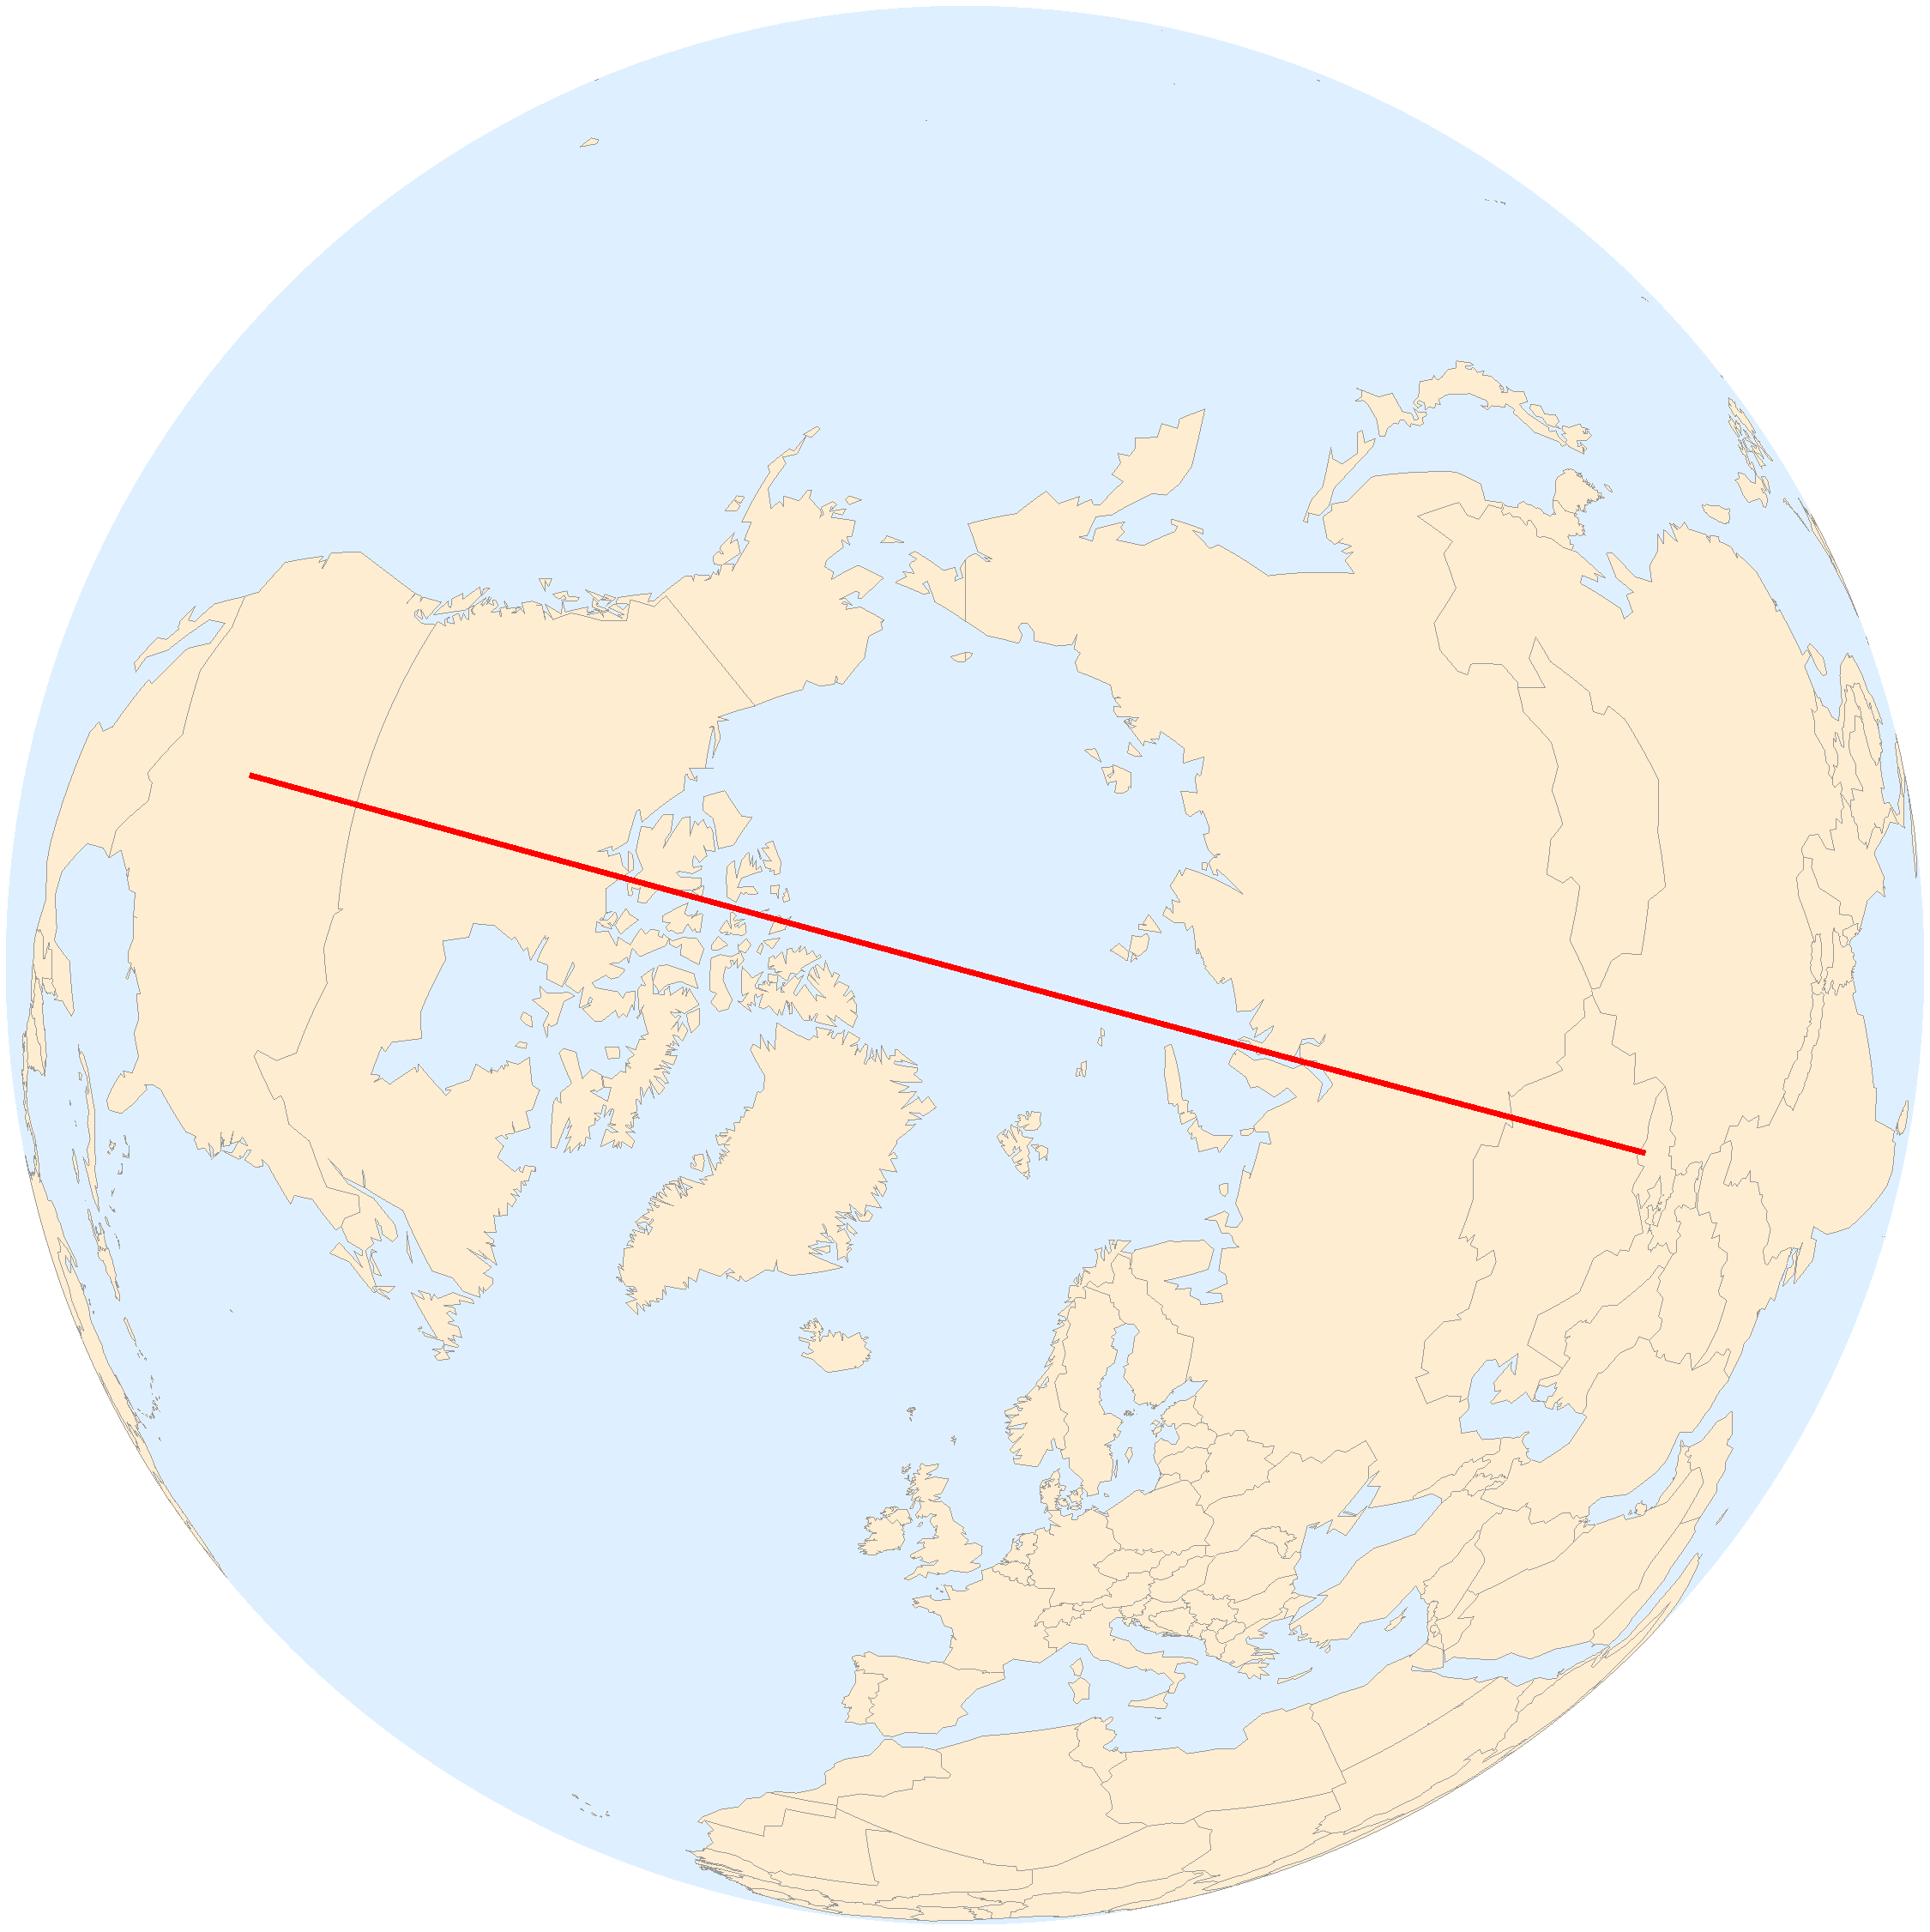
\includegraphics[width=\textwidth]{Figures/earth_two_cities.pdf}
    \end{figure}
        \vspace*{2cm}
    \end{column}
    \begin{column}{0.54\textwidth}
    \vspace*{.75cm}
       \begin{figure}[H]
        \centering
        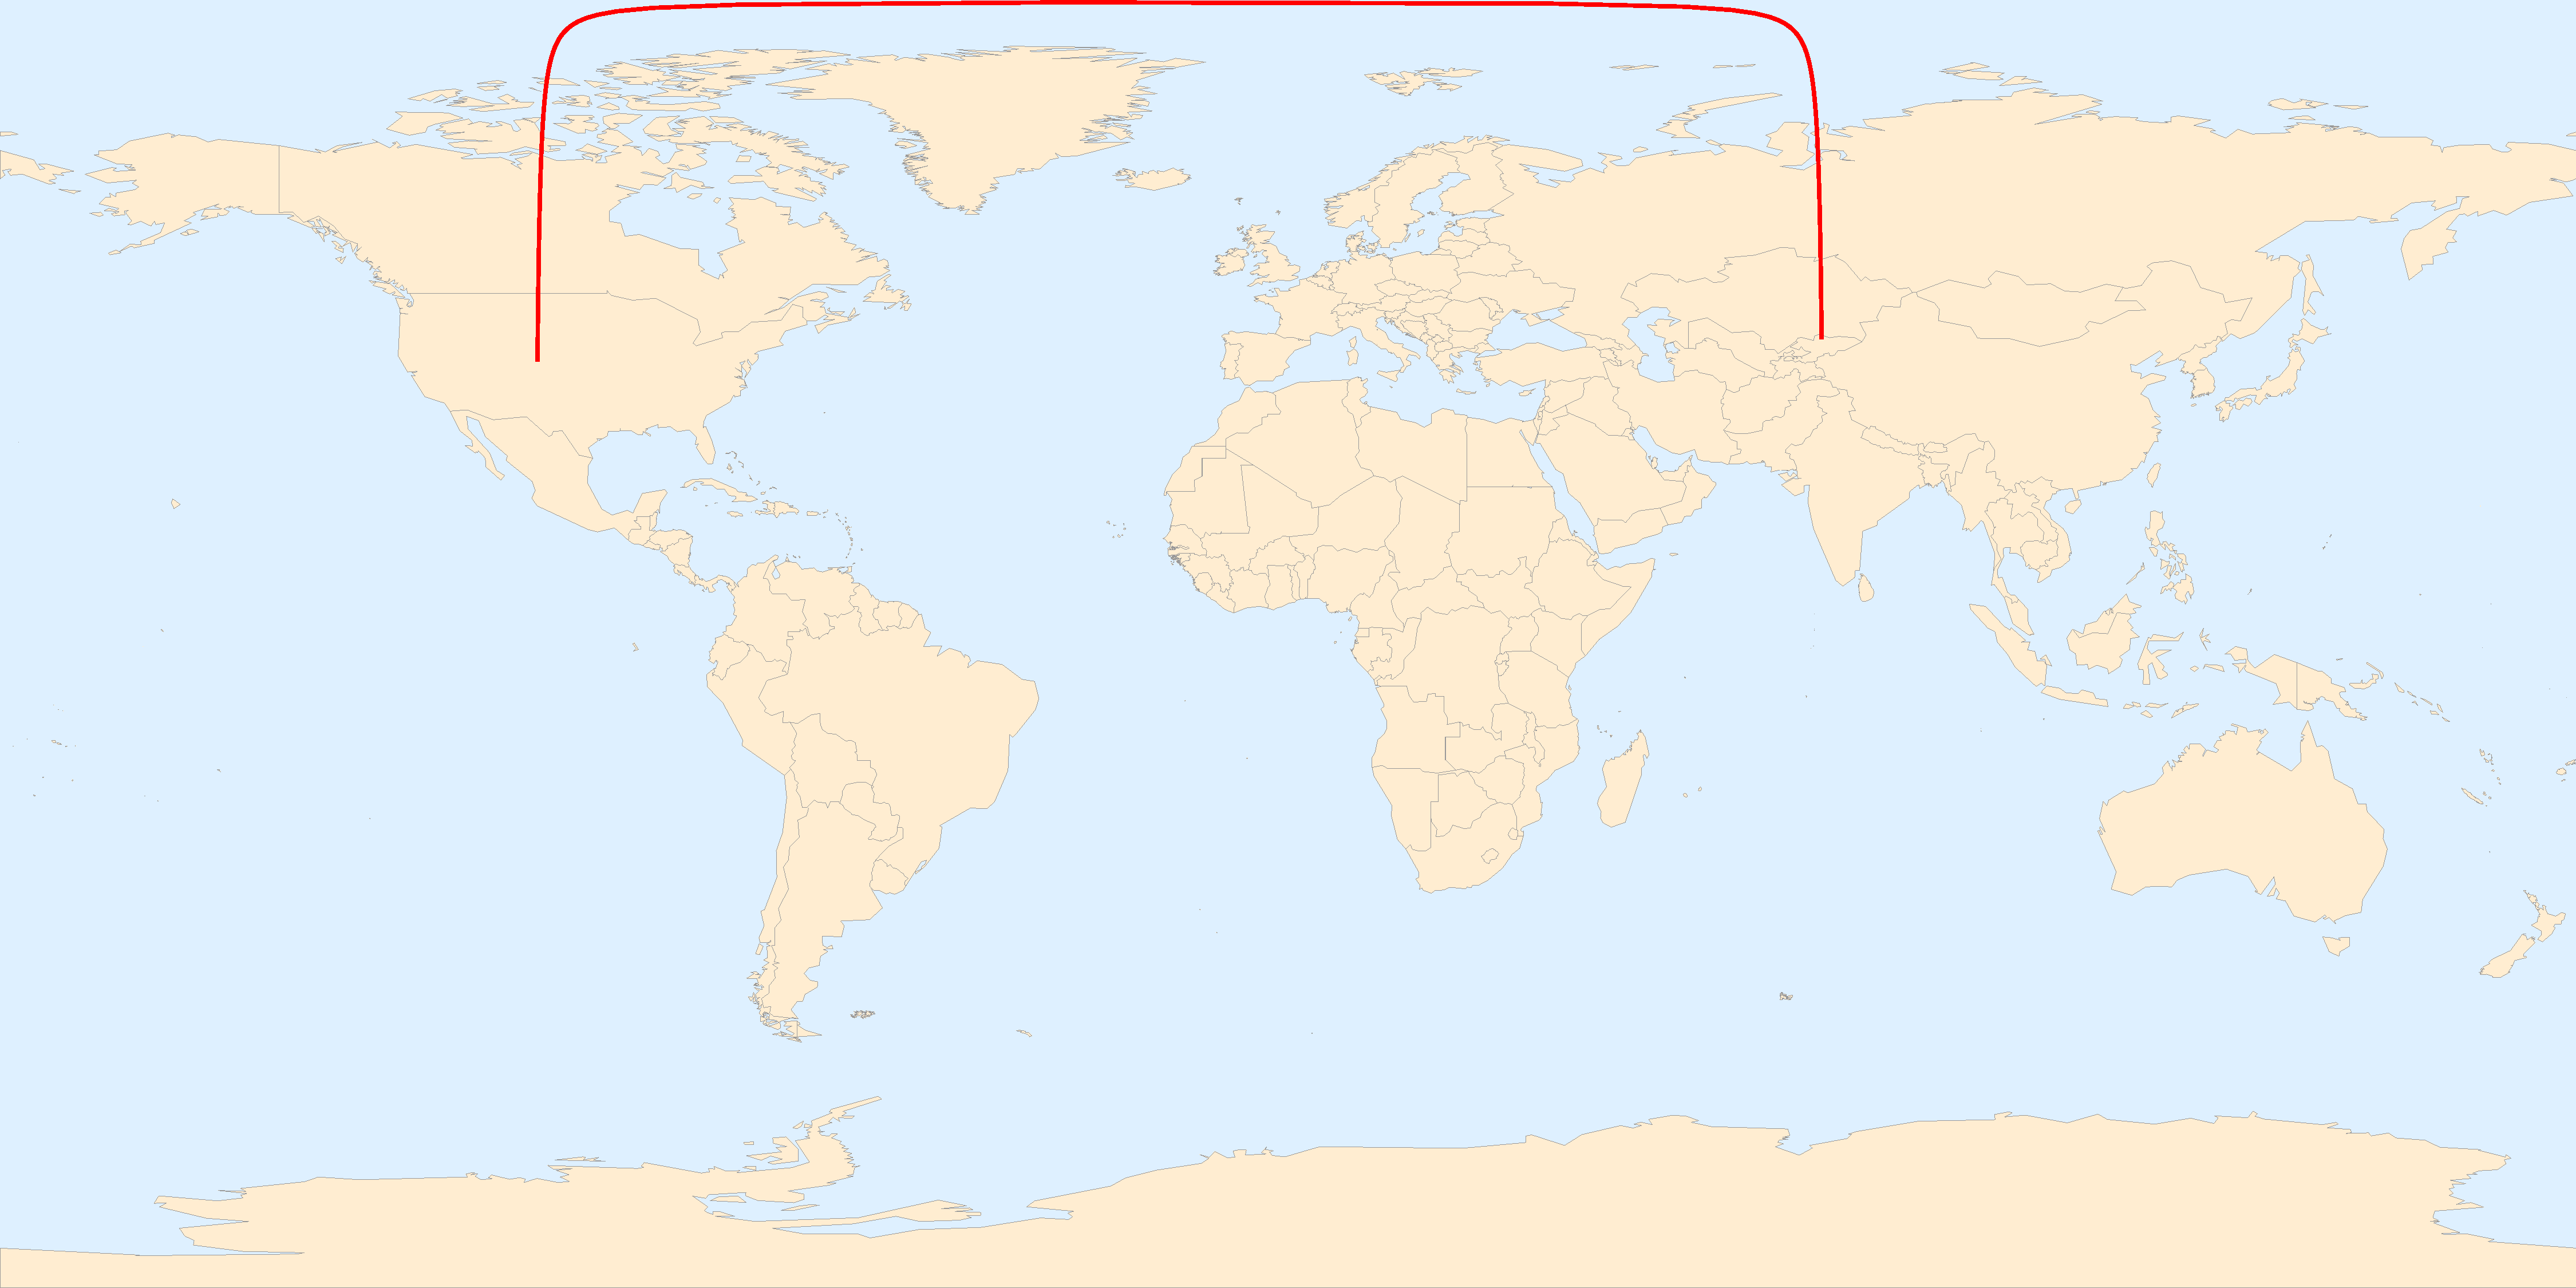
\includegraphics[width=\textwidth]{Figures/mercator_two_cities.pdf}
    \end{figure}
    \end{column}
\end{columns}
\end{frame}

\begin{frame}{Maps of Earth}
\vfill
    \begin{figure}[H]
        \centering
        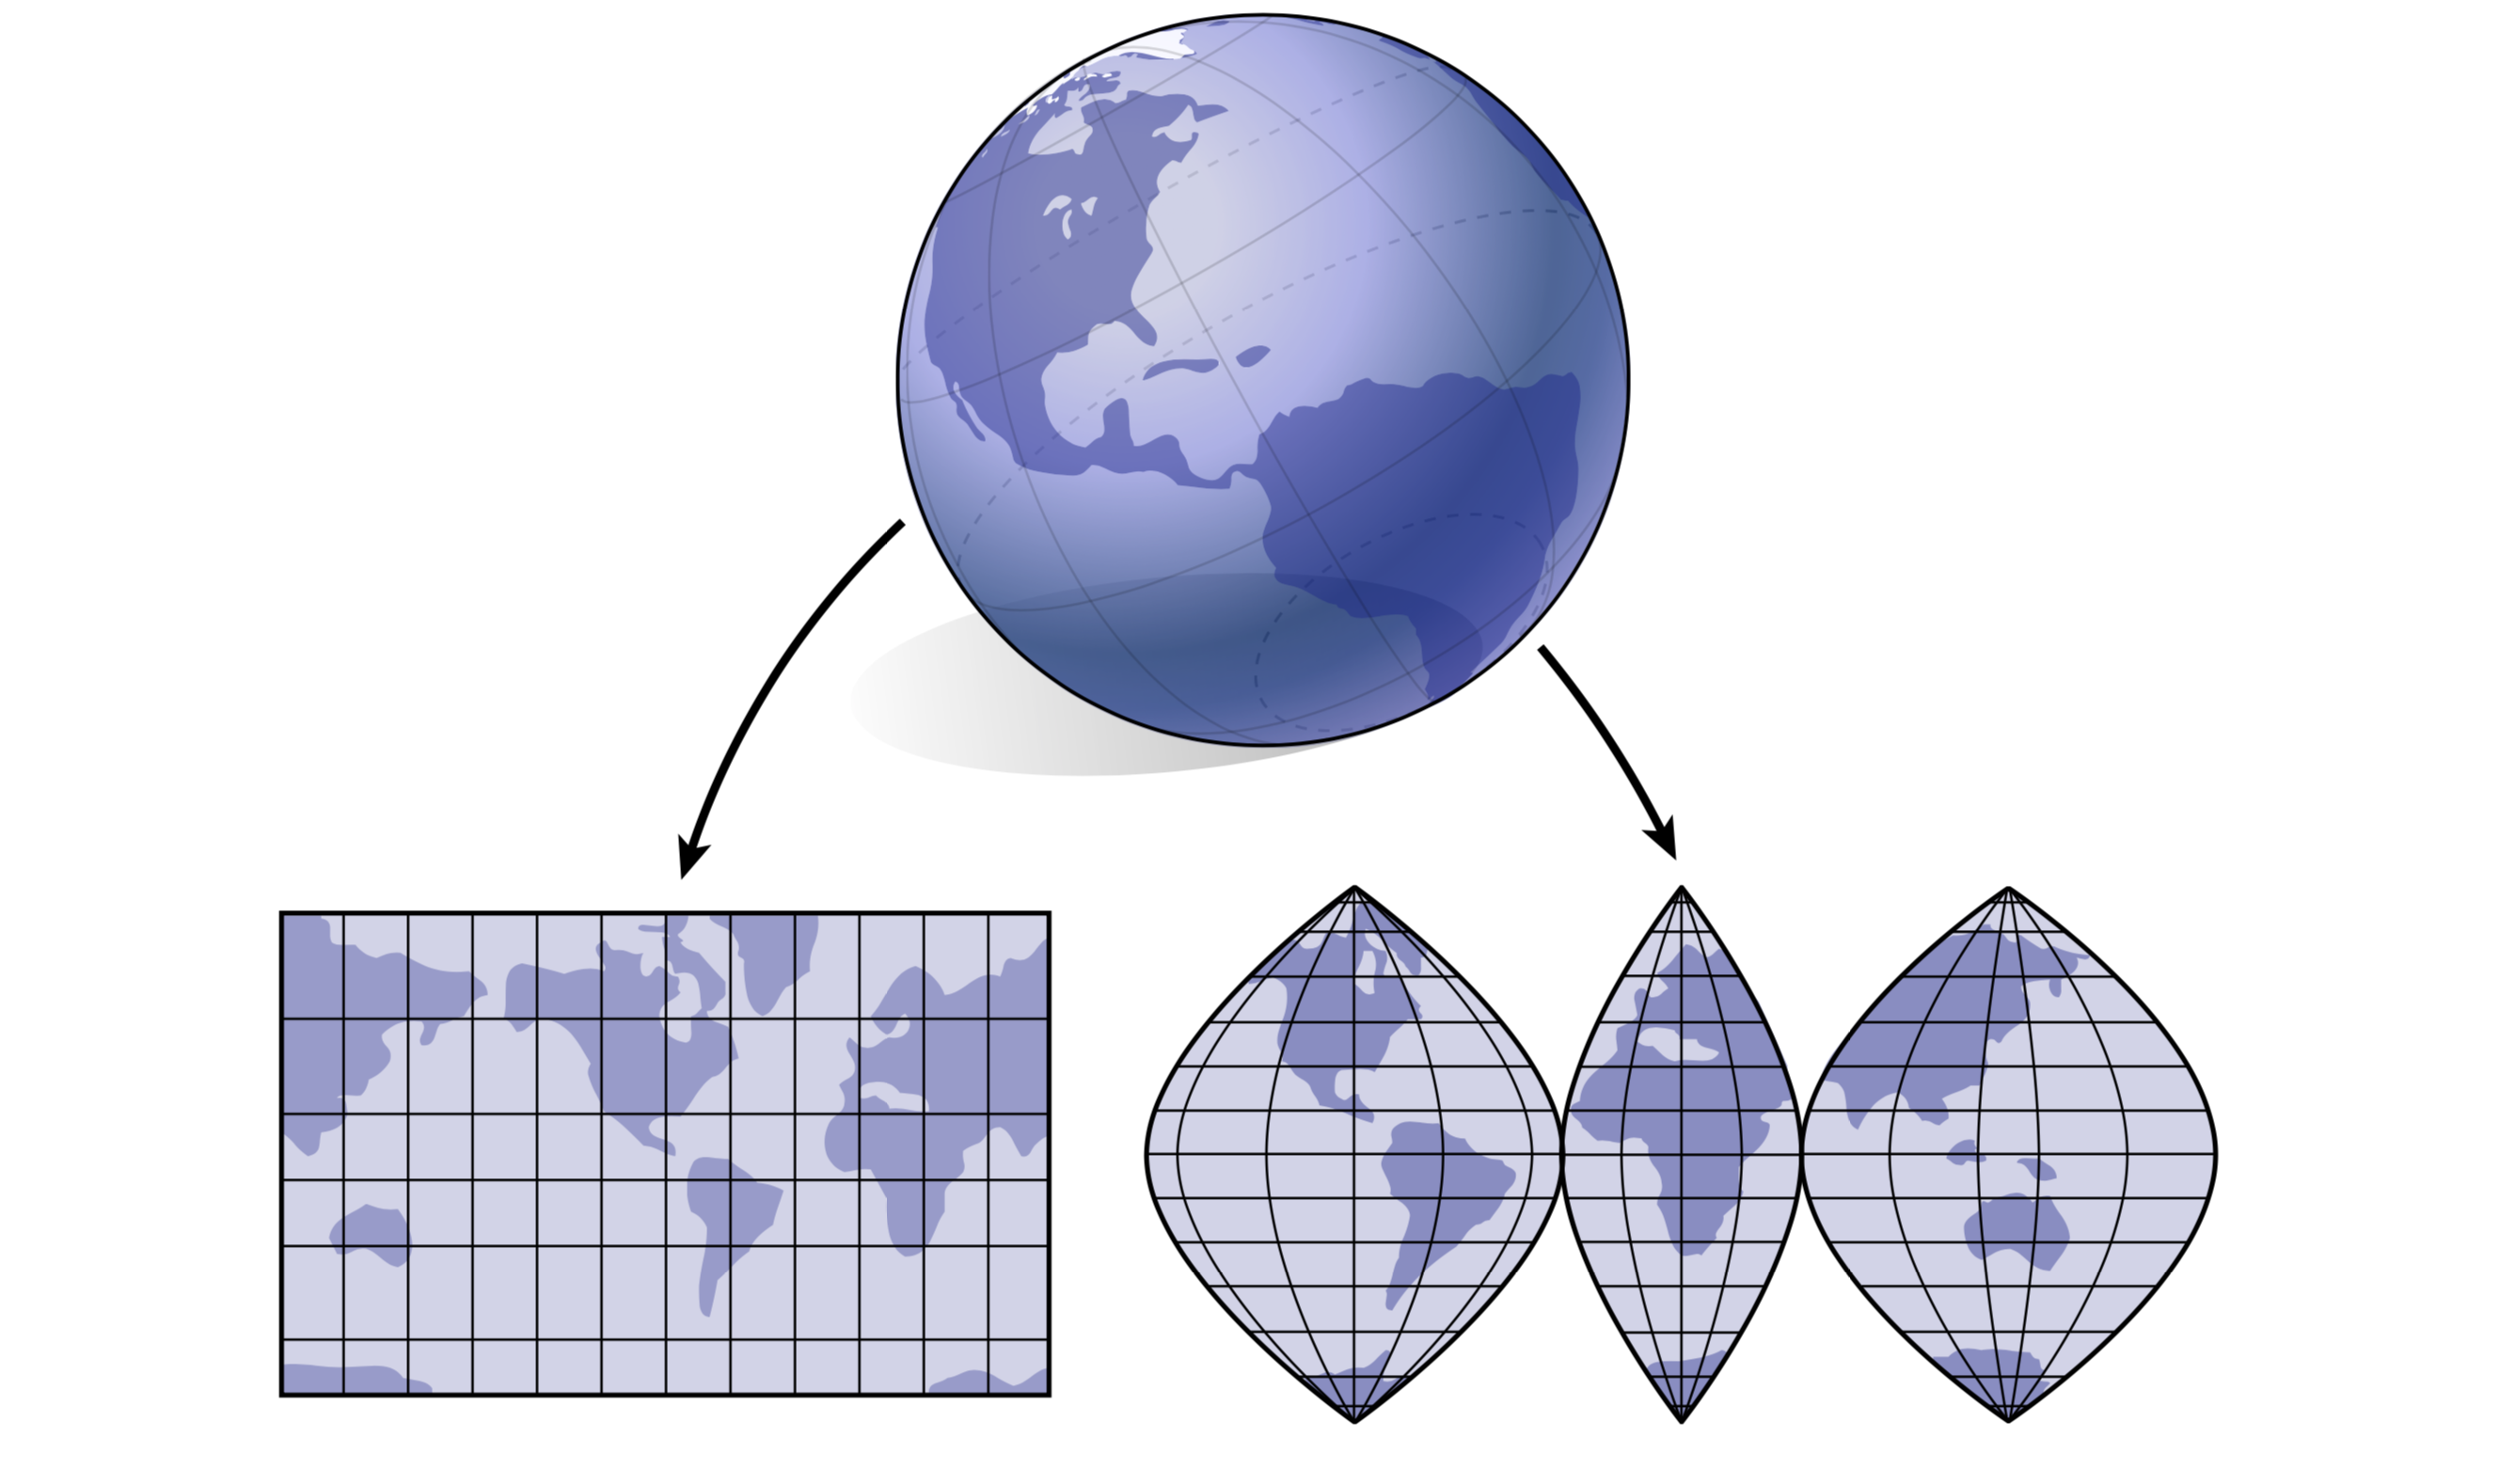
\includegraphics[width=\textwidth]{Figures/maps.png}
    \end{figure}
\end{frame}

\begin{frame}{Making a Map}
    How to make the Mercator map
    \vfill
    \begin{figure}[H]
        \centering
        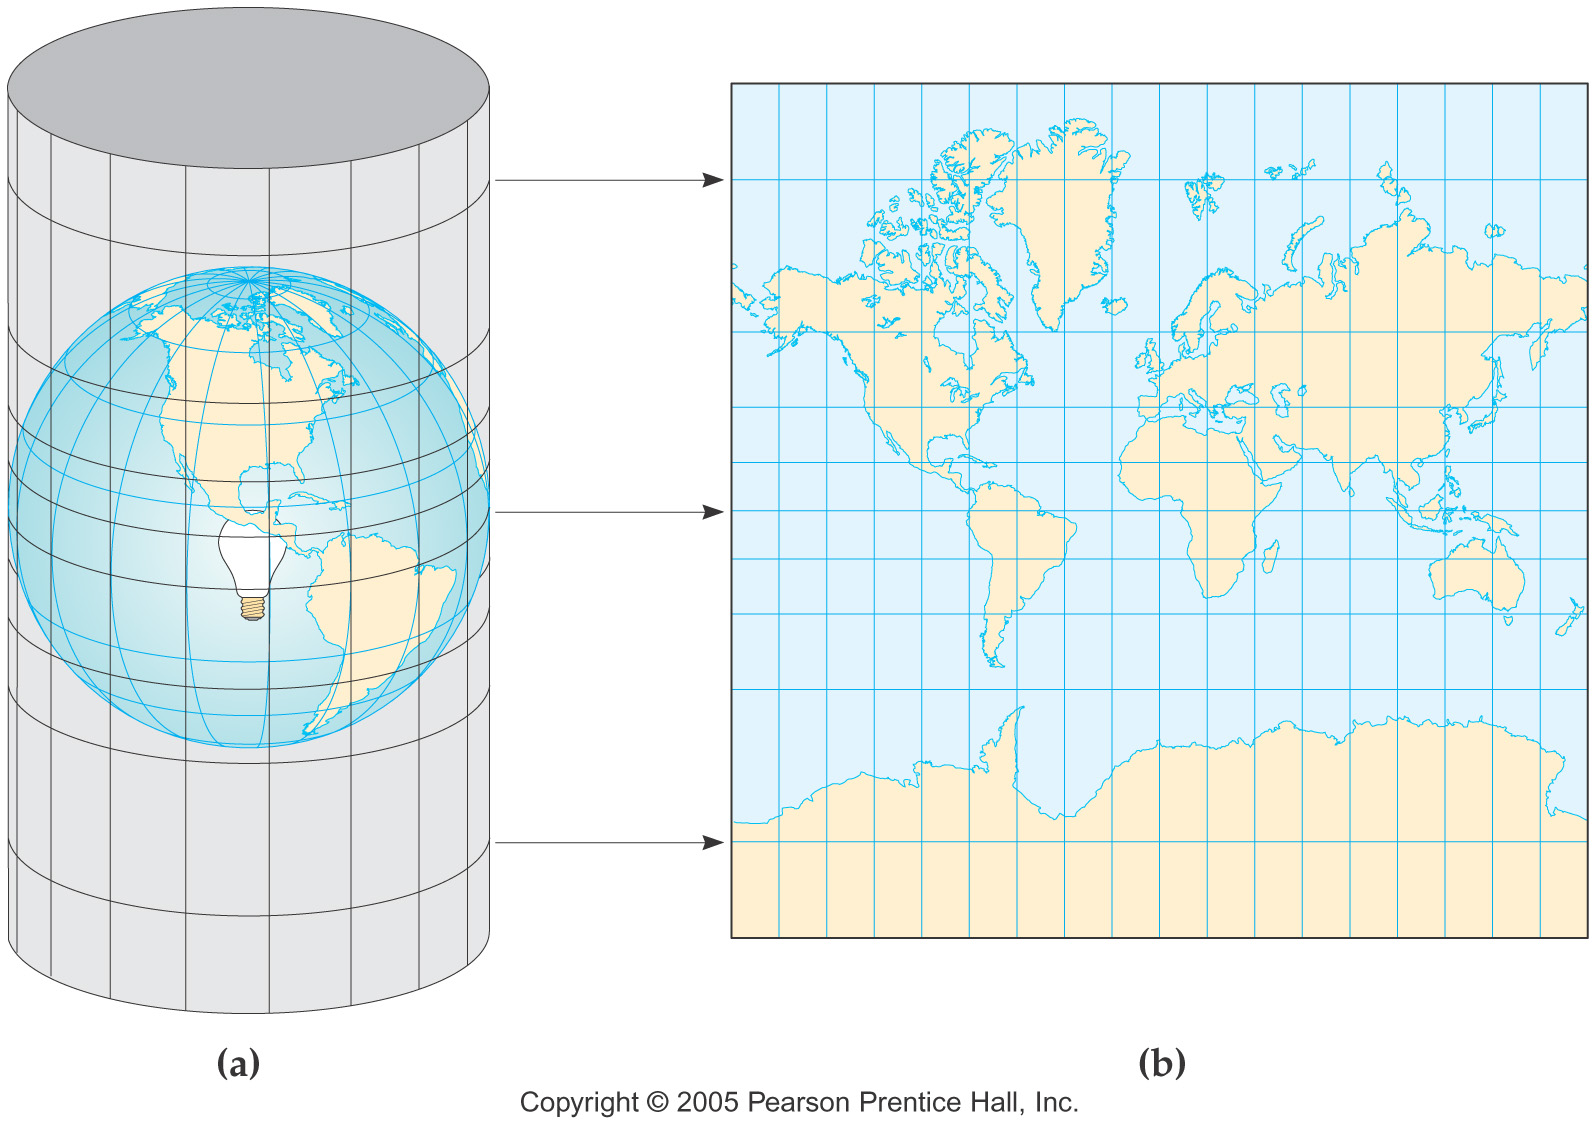
\includegraphics[width=.8\textwidth]{Figures/mercator.jpg}
    \end{figure}
\end{frame}

\end{document}